\documentclass[12pt, twoside]{article}
\usepackage[letterpaper, margin=1in, headsep=0.5in]{geometry}
\usepackage[english]{babel}
\usepackage[utf8]{inputenc}
\usepackage{amsmath}
\usepackage{amsfonts}
\usepackage{amssymb}
\usepackage{tikz}
\usetikzlibrary{quotes, angles}
\usepackage{graphicx}
\usepackage{enumitem}
\usepackage{multicol}

\newif\ifmeta
\metatrue %print standards and topics tags

\title{Regents Geometry}
\author{Chris Huson}
\date{September 2020}

\usepackage{fancyhdr}
\pagestyle{fancy}
\fancyhf{}
\renewcommand{\headrulewidth}{0pt} % disable the underline of the header
\raggedbottom


\fancyhead[LE]{\thepage}
\fancyhead[RO]{\thepage \\ Name: \hspace{4cm} \,\\}
\fancyhead[L]{BECA / Dr. Huson / Geometry 05-Transformations\\* pset ID: 63}

\begin{document}

\subsubsection*{5-6CW-Dilation-practice}
\begin{enumerate}
\item After a dilation centered at the origin, the image of $\overline{CD}$ is $\overline{C'D'}$. If the coordinates of the endpoints of these segments are $C(2,2)$, $D(4,-2)$, $C'(5,5)$, and $D'(10,-5)$, find the scale factor of the dilation.\\[0.25cm]
Make a table of coordinate pairs and graph the two line segments,  $\overline{CD}$ and  $\overline{C'D'}$, on the set of axes below.
  \begin{flushright}
    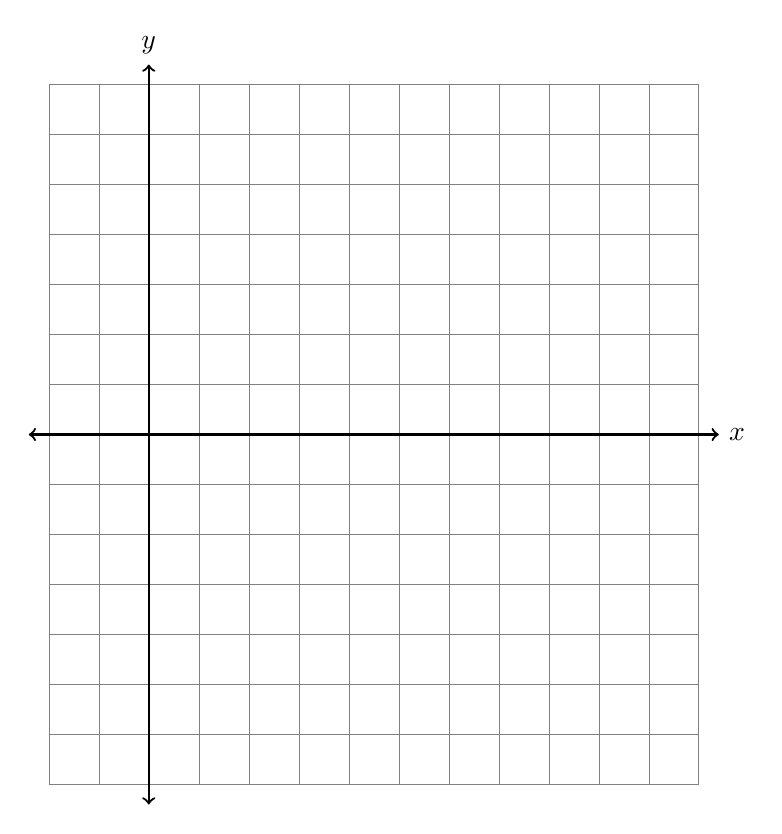
\begin{tikzpicture}[scale=.635]
      \draw [help lines] (-2,-7) grid (11,7);
      \draw [thick, <->] (-2.4,0) -- (11.4,0) node [right] {$x$};
      \draw [thick, <->] (0,-7.4)--(0,7.4) node [above] {$y$};
    \end{tikzpicture}
  \end{flushright}


\item In the diagram below of $\triangle ABC$, $D$ is a point on $\overline{BA}$, $E$ is a point on $\overline{BC}$, and $\overline{DE}$ is drawn. \\*[2pt] 
 If $BD=4$, $BA=10$, and $BE=6$, what is the length of $\overline{EC}$ so that $\overline{AC} \parallel \overline{DE}$?
 
 \begin{flushright}
     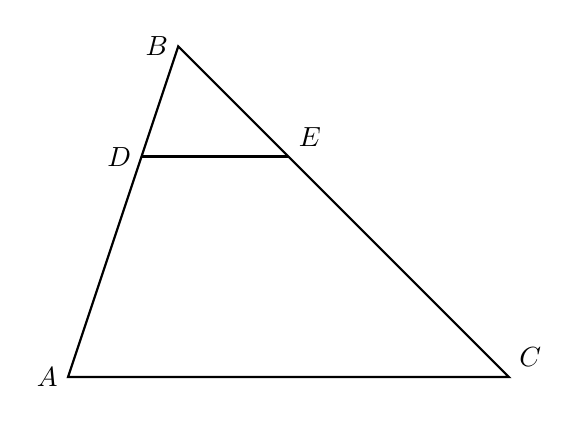
\begin{tikzpicture}[scale=0.7]
       \draw [thick]
       (0,0)node[left]{$A$}--
       (8,0)node[above right]{$C$}--
       (2,6)node[left]{$B$}--cycle;
       \draw [thick]
       (4/3,4)node[left]{$D$}--
       (4,4)node[above right]{$E$};
     \end{tikzpicture}
   \end{flushright}


\newpage


\end{enumerate}
\end{document}